%%%%%%%%%%%%%%%%%%%%%%%%%%%%%%%%%%%%%%%%%
% Beamer Presentation
% LaTeX Template
% Version 1.0 (10/11/12)
%
% This template has been downloaded from:
% http://www.LaTeXTemplates.com
%
% License:
% CC BY-NC-SA 3.0 (http://creativecommons.org/licenses/by-nc-sa/3.0/)
%
%%%%%%%%%%%%%%%%%%%%%%%%%%%%%%%%%%%%%%%%%

%----------------------------------------------------------------------------------------
%	PACKAGES AND THEMES
%----------------------------------------------------------------------------------------

\documentclass[aspectratio=149]{beamer}
\usefonttheme[onlymath]{serif}


\mode<presentation> {

% The Beamer class comes with a number of default slide themes
% which change the colors and layouts of slides. Below this is a list
% of all the themes, uncomment each in turn to see what they look like.

\usetheme{default}
%\usetheme{AnnArbor}
%\usetheme{Antibes}
%\usetheme{Bergen}
%\usetheme{Berkeley}
%\usetheme{Berlin}
%\usetheme{Boadilla}
%\usetheme{CambridgeUS}
%\usetheme{Copenhagen}
%\usetheme{Darmstadt}
%\usetheme{Dresden}
%\usetheme{Frankfurt}
%\usetheme{Goettingen}
%\usetheme{Hannover}
%\usetheme{Ilmenau}
%\usetheme{JuanLesPins}
%\usetheme{Luebeck}
%\usetheme{Malmoe}
%\usetheme{Marburg}
%\usetheme{Montpellier}
%\usetheme{PaloAlto}
%\usetheme{Pittsburgh}
%\usetheme{Rochester}
%\usetheme{Singapore}
%\usetheme{Szeged}
%\usetheme{Warsaw}

% As well as themes, the Beamer class has a number of color themes
% for any slide theme. Uncomment each of these in turn to see how it
% changes the colors of your current slide theme.

%\usecolortheme{albatross}
\usecolortheme{beaver}
%\usecolortheme{beetle}
%\usecolortheme{crane}
%\usecolortheme{dolphin}
%\usecolortheme{dove}
%\usecolortheme{fly}
%\usecolortheme{lily}
%\usecolortheme{orchid}
%\usecolortheme{rose}
%\usecolortheme{seagull}
%\usecolortheme{seahorse}
%\usecolortheme{whale}
%\usecolortheme{wolverine}

%\setbeamertemplate{footline} % To remove the footer line in all slides uncomment this line
%\setbeamertemplate{footline}[page number] % To replace the footer line in all slides with a simple slide count uncomment this line

%\setbeamertemplate{navigation symbols}{} % To remove the navigation symbols from the bottom of all slides uncomment this line
}

\usepackage{graphicx} % Allows including images
\usepackage{booktabs} % Allows the use of \toprule, \midrule and \bottomrule in tables
\usepackage{verbatim}

\usepackage{mathtools} 
\usepackage{amssymb}
\usepackage{mathrsfs}
\usepackage{amsmath}
\usepackage{bm}

\usepackage{ragged2e}
\usepackage{etoolbox}
\usepackage{lipsum}

\usepackage{siunitx,booktabs}
\usepackage{pifont}
\usepackage{array}
\usepackage{tabu,booktabs}
\usepackage{tikz}
\usetikzlibrary{arrows,shapes}

\setbeamertemplate{enumerate items}[circle]
\usepackage{tikz}

\usepackage{dsfont}

\newcommand\mynum[1]{
  \usebeamercolor{enumerate item}
  \tikzset{beameritem/.style={circle,inner sep=0,minimum size=2ex,text=enumerate item.bg,fill=enumerate item.fg,font=\footnotesize}}%
  \tikz[baseline=(n.base)]\node(n)[beameritem]{#1};
}

\newcommand\mynumm[1]{
  \usebeamercolor{enumerate item}
  \tikzset{beameritem/.style={rectangle,inner sep=0,minimum size=2ex,text=enumerate item.bg,fill=enumerate item.fg,font=\footnotesize}}%
  \tikz[baseline=(n.base)]\node(n)[beameritem]{#1};
}

\def\Put(#1,#2)#3{\leavevmode\makebox(0,0){\put(#1,#2){#3}}}

\setbeamertemplate{footline}[]

%----------------------------------------------------------------------------------------
%	TITLE PAGE
%----------------------------------------------------------------------------------------

\title{ Subsidized Housing with Slum Externalities: \\ Evidence from South Africa } % The short title appears at the bottom of every slide, the full title is only on the title page

\author{Stefano Polloni \\
joint with Ben Bradlow and Will Violette} 

 % Your institution as it will appear on the bottom of every slide, may be shorthand to save space

\date{February 2017} %\today} % Date, can be changed to a custom date

\begin{document}

\beamertemplatenavigationsymbolsempty

\begin{frame}
\titlepage % Print the title page as the first slide
\end{frame}

%\begin{frame}
%\frametitle{Overview} % Table of contents slide, comment this block out to remove it
%\tableofcontents % Throughout your presentation, if you choose to use \section{} and \subsection{} commands, these will automatically be printed on this slide as an overview of your presentation
%\end{frame}


%------------------------------------------------

%\begin{frame}
%\frametitle{Slums and Development}
%\begin{tabular}{lc} \hline
 & (1) \\
VARIABLES & Log Price \\ \hline
 &  \\
3 yrs 0-400m & -0.125 \\
 & (0.0892) \\
3 yrs 0-400m X In-Situ & 0.180 \\
 & (0.289) \\
 &  \\
Observations & 28,701 \\
R-squared & 0.489 \\
Project FE & YES \\
 Year-Month FE & YES \\ \hline
\multicolumn{2}{c}{ Robust standard errors in parentheses} \\
\multicolumn{2}{c}{ *** p$<$0.01, ** p$<$0.05, * p$<$0.1} \\
\multicolumn{2}{c}{ All control for cubic in plot size. Standard errors are clustered at the project level.} \\
\end{tabular}

%\end{frame}




%----------------------------------------------------------------------------------------
%	PRESENTATION SLIDES
%----------------------------------------------------------------------------------------
\section{Introduction}
%------------------------------------------------




\begin{frame}
\frametitle{Public Housing and Development}

% In developing countries, 30\% of urban pop live in slums (UN, 2015)

\begin{itemize}
%  \item Slum externalities $\rightarrow$ lasting poverty traps (Marx, 2013) 
%    \begin{itemize}
%      \item Poor infrastructure, high crime, health externalities
%      \item Weak incentives to invest in housing/public goods
%    \end{itemize}  
%\vspace{.2cm}
%\pause
  \item Public Housing $\rightarrow$ primary government response to slums
  \vspace{.1cm}
  \item Positive effects on direct recipients \\ 
  {\footnotesize (Cateneo et al. [2009], Franklin et al. [2016], Galiani et al. [2017])}
  \vspace{.1cm}
  \item \textbf{Question:}  What are the spillover effects of public housing in developing countries?
      \begin{itemize}
      \item \textit{Positive:} Amenity value
      \item \textit{Negative:} Crowd-in slums
    \end{itemize}
  \vspace{.1cm}
  \item \textbf{Setting:} 150+ projects in South Africa; GPS price and slum data
  \vspace{.1cm}
  \item \textbf{Findings:} Home prices drop by 16\% within 3 yrs and 400m of a project
    \begin{itemize}
      \item Home quality improves within project footprint but declines nearby (slum crowd-in)
    \end{itemize}
\end{itemize}
%    \pause

%\begin{enumerate}
%
%% ``key strategy for poverty alleviation'' {\footnotesize{South Africa}}
%%    \pause
%    \vspace{.1cm}
%\item Neighborhood Development
%  \begin{itemize}
%%    \item ``combating crime, promoting social cohesion... spatial restructuring'' South Africa Dept. of Human Settlements
%%    \pause
%%    \item \footnotesize{In US: Diamond \& McQuade [2016], Baum-Snow \& Marion [2008]}
%  \end{itemize}
%\end{enumerate}
%\begin{itemize}
%  \item \textbf{Question} \\ 
%  \vspace{.1cm}
%  What are the spillovers from public housing in developing contexts?
%\end{itemize}
%% ``combating crime, promoting social cohesion... spatial restructuring,'' {\footnotesize{South Africa}}
\end{frame}

%------------------------------------------------

% \begin{frame}
% \frametitle{This Paper}
% 
% \begin{itemize}
%   \item \textbf{Question} \\ 
%   \vspace{.1cm}
%   What are the spillovers from public housing in developing contexts?
%   \vspace{.1cm}
%     \begin{itemize}
%       \item \textbf{Positive:} Amenity value
%       \item \textbf{Negative:} Crowd-in slums
%     \end{itemize}
% 
% %\pause
% \vspace{1mm}
% \item \textbf{Approach} \\ Leverage precise timing/geography of large housing projects
% \vspace{1mm}
% \item \textbf{New Data and Setting} \\ Over 150 projects in South Africa combined with GPS property transactions and slum % growth data
% \vspace{1mm}
% \item \textbf{Initial Findings} \\ Housing projects depress home prices by 5\% within 300 meters
% \begin{itemize}
%   \item heterogeneity
%   \item ballpark estimates
% \end{itemize}
% %%%%%%%%%%%%%%%%%%%%%%%%% FIX THIS!! %%%%%%%%%%%%%%%%%%%%%%%%%%%%%%%%
% %%%%%%%%%%%%%%%%%%%%%%%%% FIX THIS!! %%%%%%%%%%%%%%%%%%%%%%%%%%%%%%%%
% %%%%%%%%%%%%%%%%%%%%%%%%% FIX THIS!! %%%%%%%%%%%%%%%%%%%%%%%%%%%%%%%%
% %%%%%%%%%%%%%%%%%%%%%%%%% FIX THIS!! %%%%%%%%%%%%%%%%%%%%%%%%%%%%%%%%
% 
% \end{itemize}
% 
% \end{frame}


%------------------------------------------------

\begin{frame}
\frametitle{Public Housing in South Africa}
  \begin{itemize}
      \item Over 4.3 million houses since 1994 (13\% of pop.)
%      \item Houses 13\% of the population
%      \item Single-story, two-room (30-40$\text{m}^2$) dwellings
      \begin{itemize}
        \item 50 to 500 houses per project
        \item Fully serviced (roads, water, sanitation, electricity)
        \item Greenfield projects on undeveloped land near slums
        \item In-Situ upgrading replacing existing slums
      \end{itemize}
     %     \begin{enumerate}
     %       \item \textbf{Greenfield projects} on undeveloped land near slums
     %       \item \textbf{In-Situ upgrading} replacing existing slums
     %     \end{enumerate}
  \end{itemize}
    %%% insert picture


\begin{itemize}
        \item Who gets a house?
          \vspace{.1cm}
      \begin{itemize}
        \item Official Policy: 
          \begin{itemize}
            \item National/provincial waiting list; no resale within 7 years
            \item Must be eligible: Citizens, new homeowners, married or dependents, inc/month $<$R3,500
          \end{itemize}
          \vspace{.1cm}
        \item In Practice:
          \begin{itemize}
            \item Waiting lists/eligibility weakly enforced
            \item Only 82\% of houses occupied by initial owners within 5 yrs
          \end{itemize}
      \end{itemize}
\end{itemize}

\end{frame}


%------------------------------------------------


%\begin{frame}
%\frametitle{Conceptual Framework}
%
%How would housing projects spillover to neighborhood outcomes?
%\vspace{.2cm}
%\begin{enumerate}
%  \item \textbf{Amenity Effect:} Upgrading housing stock/services
%    \begin{itemize}
%        \item Increase value of neighboring homes (Rossi-Hansberg [2010])
%    \end{itemize}
%\vspace{.2cm} 
%
%  \item \textbf{Crowd-In Slums:} Reduce costs of informal housing
%    \begin{itemize}
%        \item Overburden services, health/crime externalities
%        \item Reduce value of nearby houses
%    \end{itemize}
%\vspace{.2cm}
%
%  \item \textbf{Demographic Effect:} New people in the neighborhood
%    \begin{itemize}
%        \item Taste-based discrimination (Diamond and McQuade [2016])
%    \end{itemize}
%\end{enumerate}

%\begin{enumerate}
%  \item Housing externalities  {\small (Rossi-Hansberg [2010]) }
%    \begin{itemize}
%      \item Home value depends on the quality of neighboring homes
%      \item ie. informal dwellings have poor sanitation
%    \end{itemize}
%\vspace{.1cm}
%  \item Demographic externalities
%    \begin{itemize}
%      \item Taste-based discrimination
%      \item Overcrowding $\rightarrow$ crime/health externalities
%    \end{itemize}
%\vspace{.1cm}
%  \item Access to public goods (water, sewer, road infrastructure)
%\end{enumerate}
%\end{frame}



%------------------------------------------------



\begin{frame}
\frametitle{Measuring Public Housing and Spillovers}

\begin{itemize}
  \item Focus on Gauteng Province (includes Johannesburg and Pretoria)
\end{itemize}

\begin{enumerate}
\item \textbf{Property Transactions} 500,000 deeds records (bottom 20\% of formal housing market)
  \begin{itemize}
    \item Buyer/seller name, GPS, price, date from 2002-2011
  \end{itemize}
\vspace{.1cm}
\item \textbf{Building Census:} GPS for over 4 mil. buildings in 2001 and 2011
\vspace{.1cm}
\item \textbf{Population Census:} in 2001 and 2011
\vspace{.1cm}
\item \textbf{Admin. Project Records:} location, dates, costs
  \begin{itemize}
    \item Includes planned but unconstructed projects
  \end{itemize}
\end{enumerate}

\end{frame}

%------------------------------------------------

\begin{frame}
\frametitle{Identifying Housing Projects}

Completed projects:
\begin{itemize}
\item Use sales from government sellers on previously empty land plots
\item Cluster sales into projects based on geographic proximity
\item Include projects where over 50\% of sales occurred in the same year
\end{itemize}

\end{frame}





%  
%  
%  \item \textbf{Temporal Clustering:} include cluster with $>$50\% of transactions during modal year


\begin{frame}
\frametitle{Identifying Housing Projects}

\begin{tikzpicture}[overlay]

\onslide<1->\node[overlay,anchor=west,align=left] at (0, 2.5) {    \begin{minipage}{1\textwidth} {\begin{enumerate}
  \item \textbf{Seller Identity:} match government names and housing authorities in seller-names from transactions 
\end{enumerate}}\end{minipage}};

\onslide<2->\node[overlay,anchor=west,align=left] at (0, 1.5) {    \begin{minipage}{1\textwidth} { 
\begin{enumerate}
  \setcounter{enumi}{1}
  \item \textbf{Subsidy Value:} exclude purchase prices R50,000 above subsidy value ($<$4\% of remaining transactions)
\end{enumerate}}\end{minipage}};

\onslide<3->\node[overlay,anchor=west,align=left] at (0, .5) {    \begin{minipage}{1\textwidth} { 
\begin{enumerate}
  \setcounter{enumi}{2}
  \item \textbf{Pre-Existing Formal Dwellings:} exclude land plots with formal structures in 2001 building census (31\% of remaining transactions)
\end{enumerate}}\end{minipage}};

\onslide<4->\node[overlay,anchor=west,align=left] at (0, -.5) {    \begin{minipage}{1\textwidth} { 
\begin{enumerate}
  \setcounter{enumi}{3}
  \item \textbf{Spatial Clustering:} collect nearby houses into projects with density-based clustering algorithm
\end{enumerate}}\end{minipage}};

\onslide<5->\node[overlay,anchor=west,align=left] at (0, -1.5) {    \begin{minipage}{1\textwidth} { 
\begin{enumerate}
  \setcounter{enumi}{4}
  \item \textbf{Temporal Clustering:} include clusters with $>$50\% of transactions during modal year (\%50 of clusters)
\end{enumerate}}\end{minipage}};

\onslide<5->\node[overlay,anchor=west,align=left] at (0, -2.6) {    \begin{minipage}{1\textwidth} { 
\begin{itemize}
  \item Overlaps well with completed projects from admin. data
\end{itemize}}\end{minipage}};



\onslide<1>\node[overlay,anchor=west,align=left] at (0, -1) {
\begin{minipage}{1\textwidth} { 
\begin{figure}
\caption{Top 5 Seller Names}
\begin{tabu}{lc}
\toprule
 Seller Name & Observations \\
\midrule
City Of Johannesburg Metropolitan Municipality & 29,087  \\
City Of Johannesburg & 27,672  \\
City Of Tshwane Metropolitan Municipality & 24,780  \\
Ekurhuleni Metropolitan Municipality & 21,758  \\
Gauteng Provincial Housing Advisory Board & 13,058  \\
{\bf Total Observations }& {\bf 549,704}  \\
\bottomrule
\end{tabu}
 
\end{figure}
}\end{minipage}
} ;
% descriptive_statistics.do   program: write_biggest_sellers


\onslide<2>\node[overlay,anchor=west,align=left] at (0, -2) { 
\begin{minipage}{1\textwidth} { 
\begin{figure}
\caption{Purchase Price Densities}
 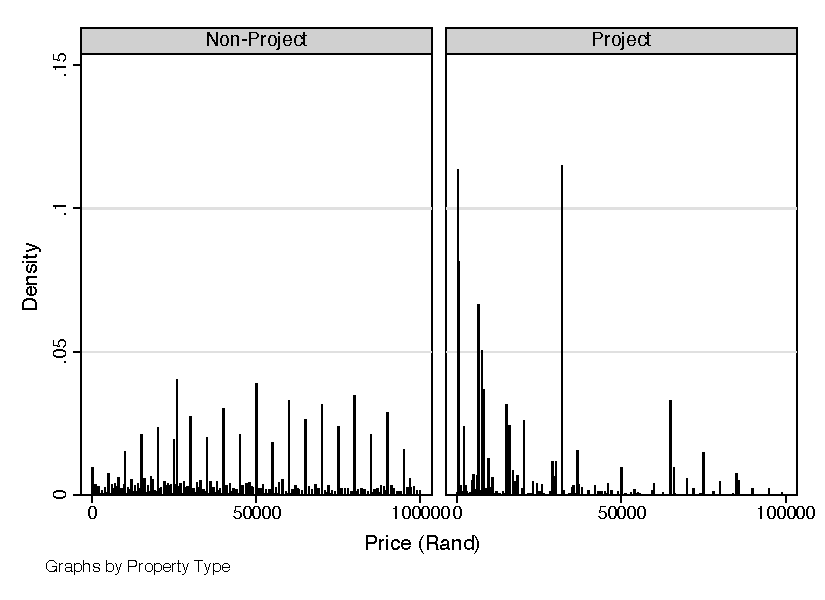
\includegraphics[scale=.5]{price_histogram.pdf} 
\end{figure}
}\end{minipage} 
} ;
% descriptive_statistics.do   program: write_price_histogram


\onslide<4>\node[overlay,anchor=west,align=left] at (2, -2.8) {  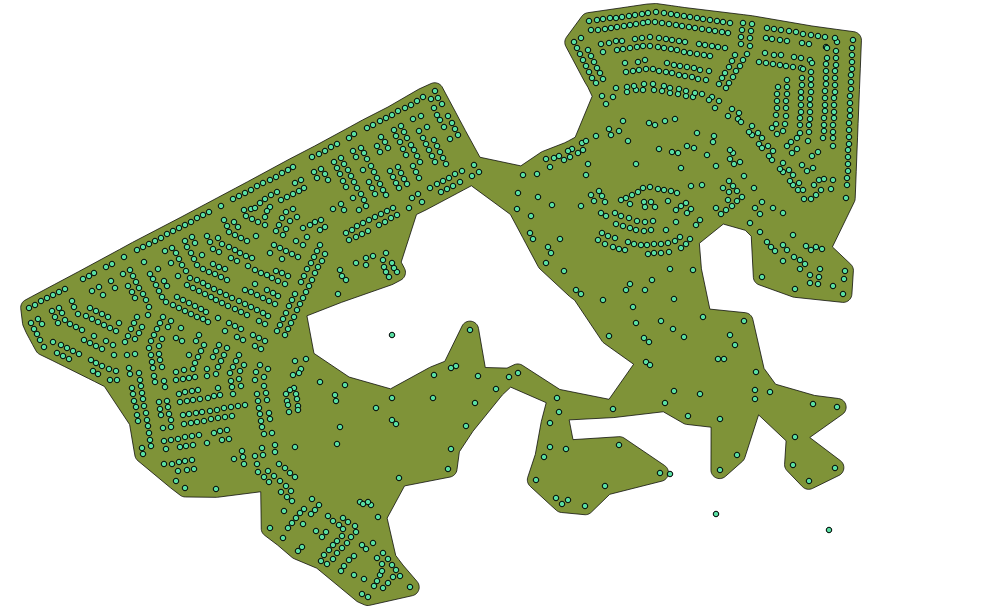
\includegraphics[scale=.16]{rdp_conhull_pic.png}  };
% generated from QGIS


\end{tikzpicture}

\end{frame}





%------------------------------------------------


\begin{frame}
\frametitle{Identifying Planned but Unconstructed Projects}

\begin{enumerate}
  \item Admin. data have ``planned,'' ``proposed,'' ``implementing'' projects
    \begin{itemize}
      \item Exclude projects with identified project transactions
    \end{itemize}

    \vspace{.2cm}

  \item Assign projects an expected completion date
    \begin{itemize}
      \item Fuzzy-string match budget data (with start-dates) on project names
      \item Add avg. diff. between transaction-date and start-date for completed projects
    \end{itemize}
\end{enumerate}

\begin{itemize}
  \item Why are projects canceled/delayed? 
    \begin{itemize}
      \item Legal disputes, service delivery backlogs, funding complications
      \item Delays often exceed 12 years 
    \end{itemize} 
\end{itemize}
\end{frame}

%------------------------------------------------

\begin{frame}
\frametitle{Housing Projects}
\begin{center}
\begin{tabu}{lcc}
 & Completed & Uncompleted \\ 
 Formal Density: 2001  & 340.6  & 89.1  \\ 
 Formal Density: 2011  & 1,783.1  & 491.1  \\ 
 &  &  \\ 
 Informal Density: 2001  & 443.0  & 1,569.2  \\ 
 Informal Density: 2011  & 1,064.6  & 1,993.4  \\ 
 &  &  \\ 
 Median Year (est.)  & 2005  & 2007  \\ 
 Distance to CBD (km)  & 28.9  & 27.6  \\ 
 &  &  \\ 
 Total Projects   & 56  & 35  \\ 
\bottomrule
\end{tabu}

\end{center}
Home counts are from building census.
\end{frame}



%-------------------- BUILDING COUNTS --------------
\begin{frame}
\frametitle{How do projects affect housing growth?}
\begin{itemize}
  \item Count structures within 50 by 50 meter grids
\end{itemize}
\begin{center}
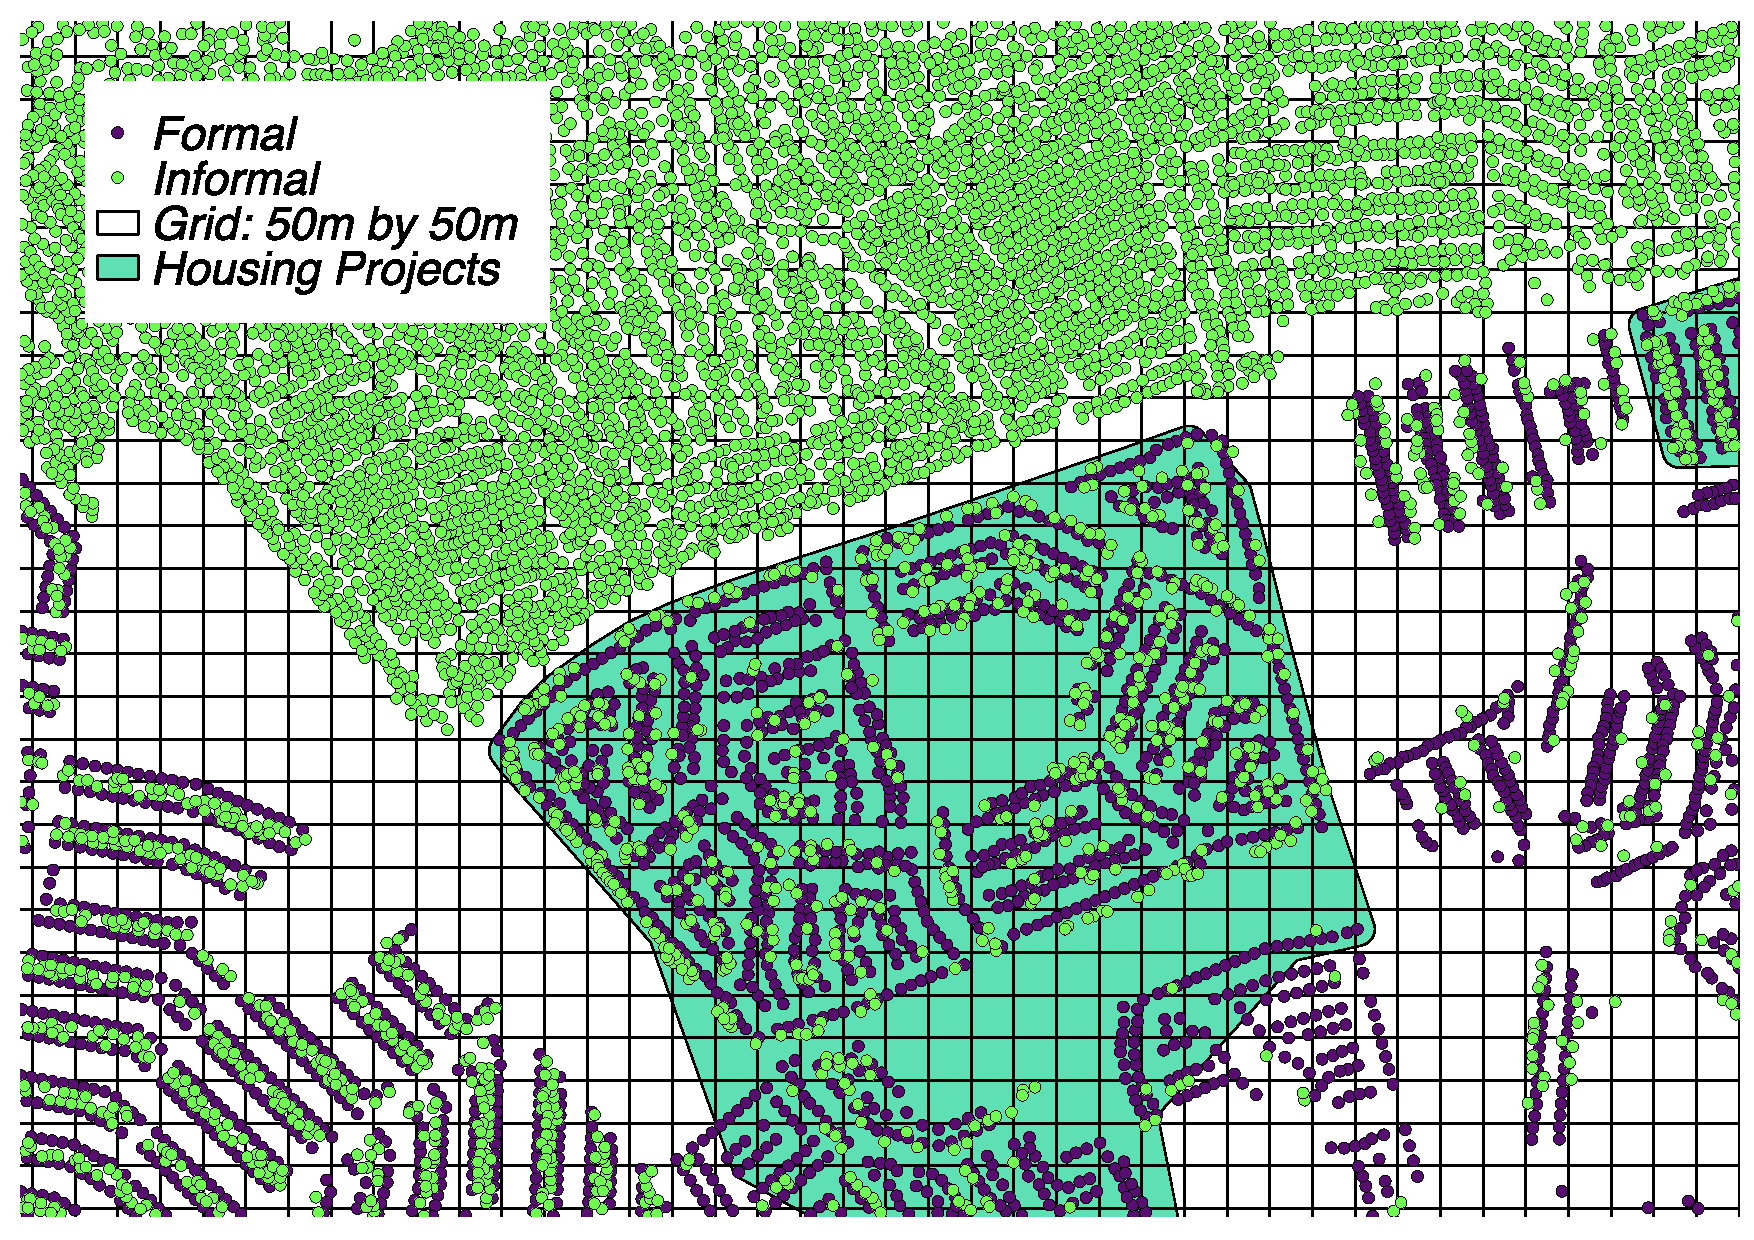
\includegraphics[scale=0.33]{bblu_map.pdf}
\vspace{-3mm}
\end{center}
\end{frame}

%------------------------------------------------

\begin{frame}
\frametitle{Estimating Differences-in-Differences}

\begin{align*}
H_{gtp} \, &= \, \sum_{d=1}^{D} \alpha_d \mathds{1}[dist=d] Post_{tp} C_p + \sum_{d=1}^{D} \beta_d \mathds{1}[dist=d] Post_{tp} U_p   \\
& +  \lambda_g \, + \, \varepsilon_{gtp}
\end{align*}

\begin{itemize}
\item $g$: grid cell, $t$: year (2001, 2011), $p$: project
\item $H_{gtp}$: Houses per grid cell
\item $dist$: distance from boundary ($<0$ within project)
\item $Post_{tp}$: After project
\item $C_{bp}$: Completed, $U_{bp}$: Uncompleted
\item $\lambda_g$: grid cell fixed effect
\end{itemize}

\begin{itemize}
  \item \textbf{Identification}: Counterfactual outcomes for completed projects would have changed in the same way as uncompleted projects.
\end{itemize}

\end{frame}

%------------------------------------------------

%\begin{frame}
%\frametitle{All Houses}
%\begin{center}
%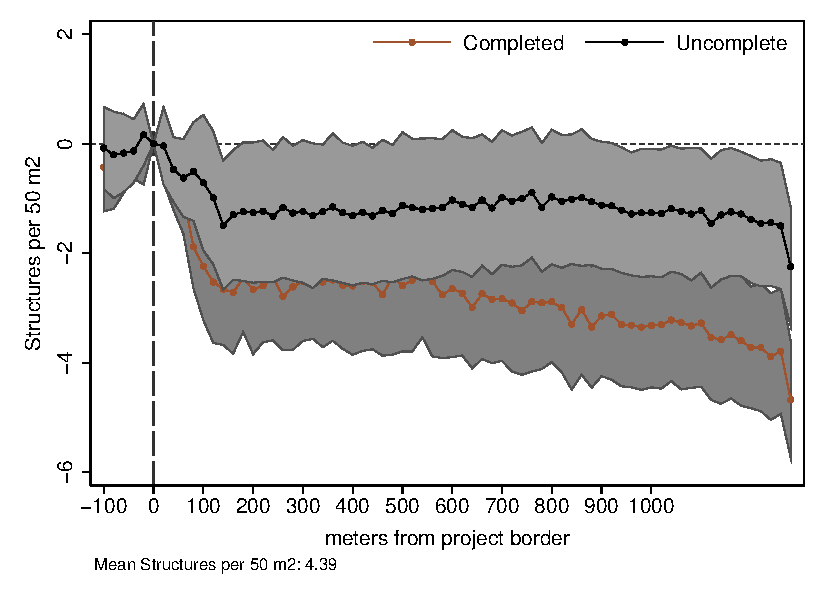
\includegraphics[scale=.78]{distplot_bblu_b.pdf}
%\vspace{-3mm}
%\end{center}
%\end{frame}

\begin{frame}
\frametitle{Formal Houses}
\begin{center}
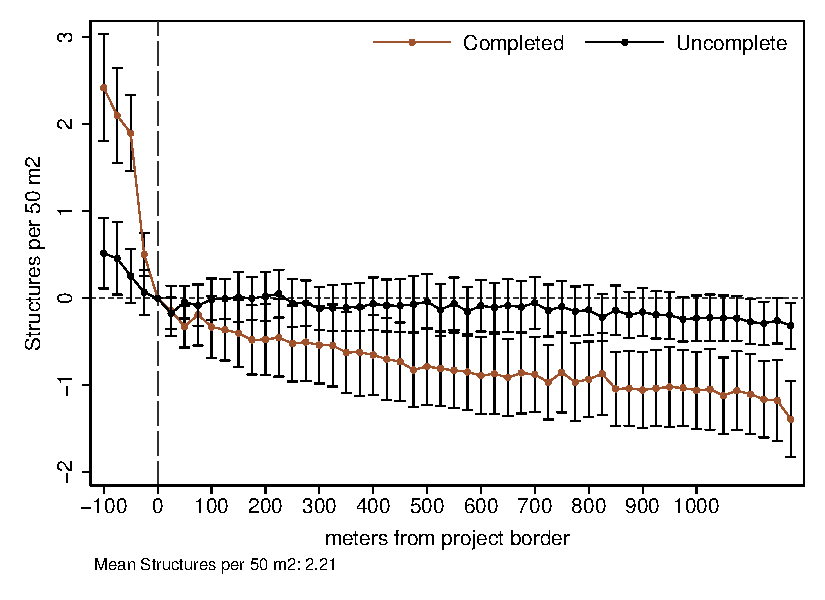
\includegraphics[scale=.78]{distplot_bblu_for.pdf}
\vspace{-3mm}
\end{center}
\end{frame}

\begin{frame}
\frametitle{Informal Houses (Slums)}
\begin{center}
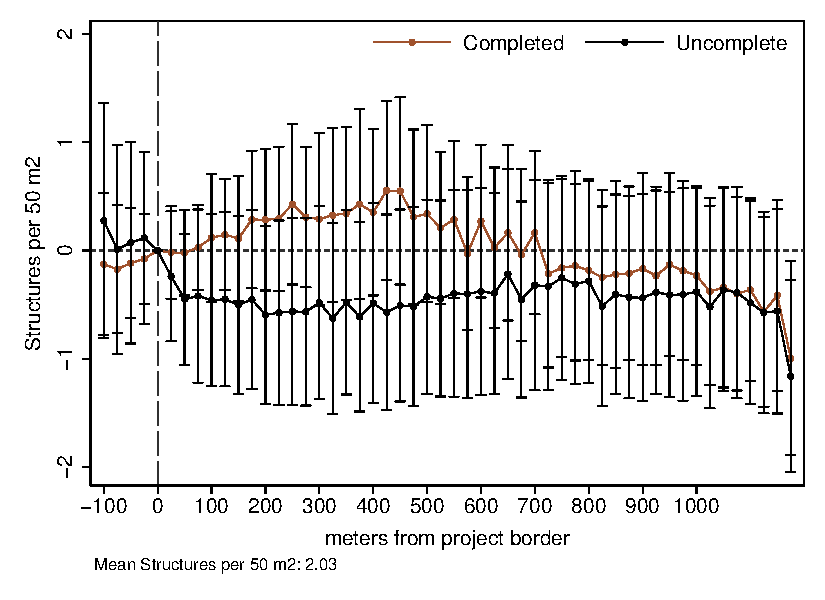
\includegraphics[scale=.78]{distplot_bblu_inf.pdf}
\vspace{-3mm}
\end{center}
\end{frame}

\begin{frame}
\frametitle{Commercial Buildings}
\begin{center}
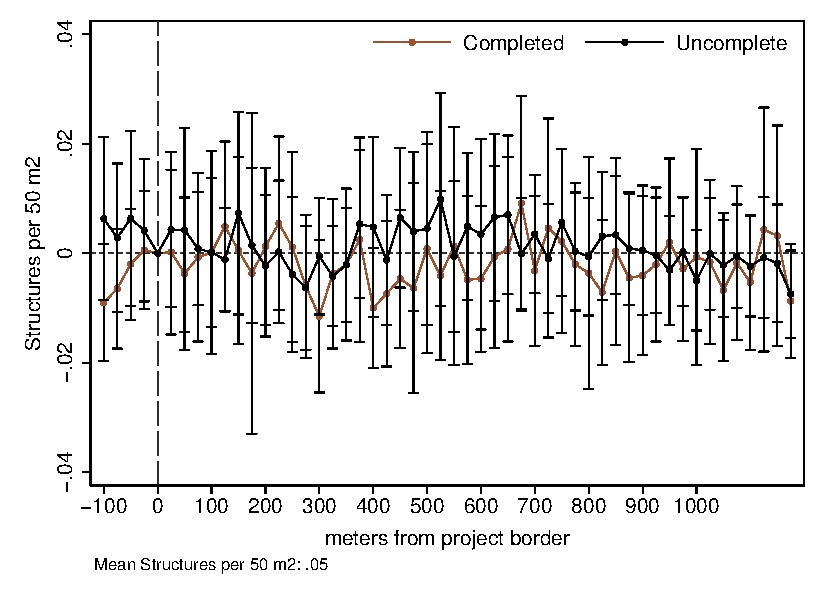
\includegraphics[scale=.78]{distplot_bblu_shops.pdf}
\vspace{-3mm}
\end{center}
\end{frame}

%---------------------  CENSUS EFFECTS  ---------------------------

\begin{frame}
\frametitle{How do projects affect census demographics?}
\begin{itemize}
  \item Project Blocks: $>$30\% overlap (yellow)
  \item Spillover Blocks: $<$30\% overlap, centroids within 1.2 km (blue)
\end{itemize}
\begin{center}
\begin{figure}
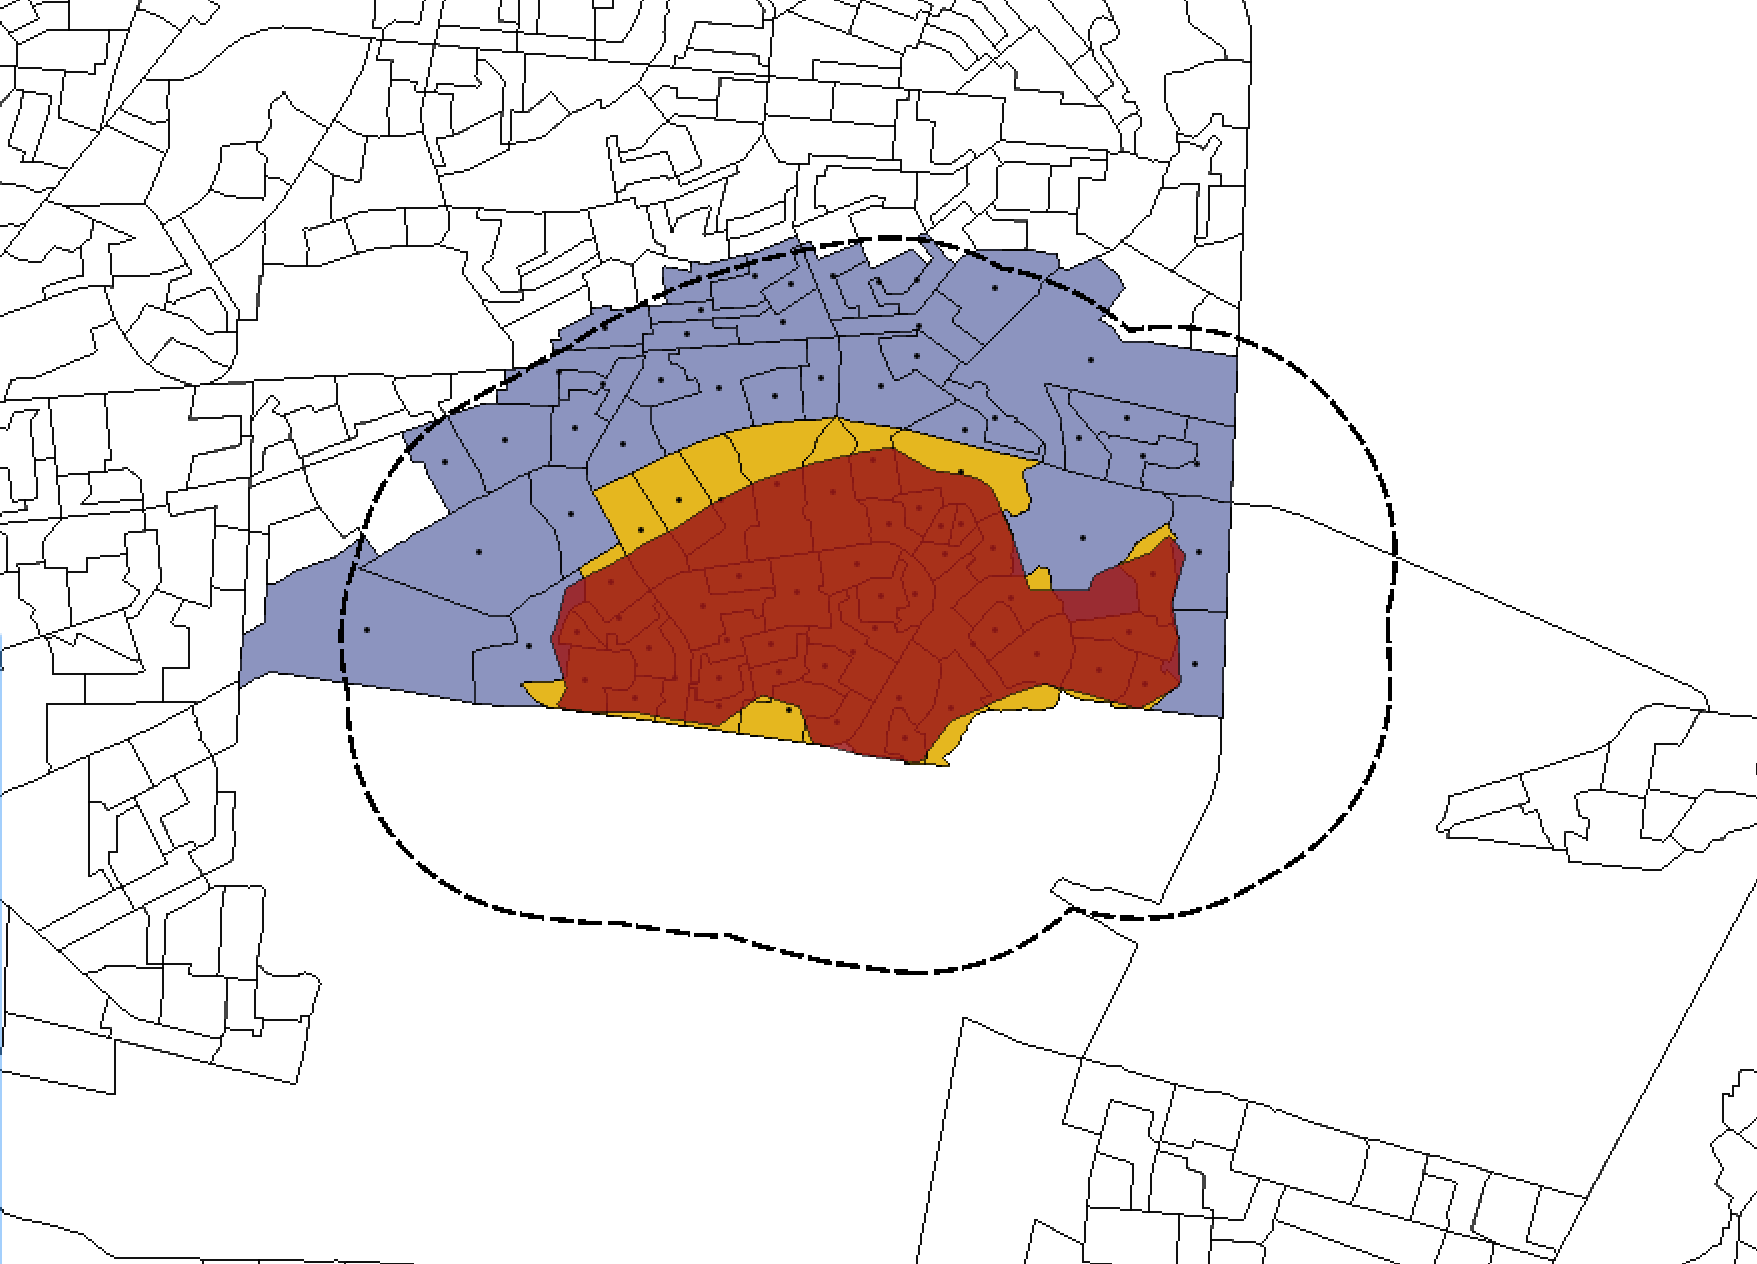
\includegraphics[scale=0.27]{design_7.png}
\vspace{-3mm}
\end{figure}
\end{center}
\end{frame}



%------------------------------------------------

\begin{frame}
\frametitle{Census Descriptives at Baseline (2001)}
\begin{itemize}
    \item Uncompleted project areas have worse outcomes
    \item Spillover areas are comparable
\end{itemize}
\vspace{.1cm}
\centering
\resizebox{\textwidth}{!}{  
\begin{tabu}{lcccc}
 & \multicolumn{2}{c}{Within Project}     & \multicolumn{2}{c}{Outside Project}    \\
 & \multicolumn{2}{c}{($>$30\% Overlap)}  & \multicolumn{2}{c}{($<$30\% Overlap)}   \\
 &  &  &  &  \\ 
 & Completed & Uncompleted & Completed  & Uncompleted  \\
\midrule
 Flush Toilet  & 0.56  & 0.18  & 0.77  & 0.82  \\ 
 &  &  &  &  \\ 
 Piped Water  & 0.21  & 0.07  & 0.41  & 0.36  \\ 
 &  &  &  &  \\ 
 Elec. Cooking  & 0.58  & 0.17  & 0.68  & 0.68  \\ 
 &  &  &  &  \\ 
 Elec. Light  & 0.79  & 0.23  & 0.74  & 0.82  \\ 
 &  &  &  &  \\ 
 Single House  & 0.51  & 0.45  & 0.52  & 0.59  \\ 
 &  &  &  &  \\ 
\midrule
 Observations  & 59,460  & 37,136  & 213,061  & 194,622  \\ 
\bottomrule
\end{tabu}

}
% descriptive_statistics.do program: write_census_hh_table
\end{frame}


%------------------------------------------------



\begin{frame}
\frametitle{Census Difference-in-Differences}
\begin{align*}
Y_{hbtp} \, &= \, \alpha_{1} \, Post_{tp}\,  C_{bp}\,  Project_{bp} \, + \alpha_{2} \, Post_{tp} \, C_{bp} \, Spillover_{bp} \,   \\
&\\
&+ \,\theta_1\,  Post_{tp} \, Project_{bp} + \,\theta_2 \, Post_{tp} \, Spillover_{bp}  \,  \\
&\\
& + \theta_3\,  C_{bp} \, Spillover_{bp} \, +  \, \theta_4 \, Spillover_{bp} \, +  \lambda_p \, + \, \varepsilon_{hbtp}
\end{align*}

\begin{itemize}
\item $h$: household, $b$: census block, $t$: year (2001, 2011), $p$: project
\item $Post_{tp}$: After project
\item $C_{bp}$: Completed
\item $Project_{bp}$: $>$\%30 overlap
\item $Spillover_{bp}$: $\leq$\%30 overlap
\item $\lambda_p$: Project fixed effect
\end{itemize}

\begin{itemize}
  \item \textbf{Identification}: Counterfactual outcomes for completed projects would have changed in the same way as uncompleted projects.
\end{itemize}


% descriptive_statistics.do program: write_census_hh_table
\end{frame}



%------------------------------------------------



\begin{frame}
\frametitle{Census Differences-in-Differences Estimates}

\resizebox{\textwidth}{!}{  
\begin{tabular}{lcccc} \hline
 & (1) & (2) & (3) & (4)  \\
VARIABLES & Flush Toilet & Piped Water Inside & Electric Cooking & Electric Lighting \\ \hline
 &  &  &  &   \\
Project X Post X Complete & 0.210** & 0.202*** & 0.0679 & -0.0482 \\
 & (0.0824) & (0.0540) & (0.0849) & (0.0998)  \\
 Spillover X Post X Complete & -0.0723* & -0.0464 & -0.130*** & -0.0461 \\
 & (0.0411) & (0.0302) & (0.0449) & (0.0385)  \\
Project X Post & 0.115** & 0.148*** & 0.353*** & 0.270***  \\
 & (0.0448) & (0.0298) & (0.0760) & (0.0822)  \\
Spillover X Post & 0.136*** & 0.182*** & 0.268*** & 0.138***  \\
 & (0.0313) & (0.0205) & (0.0347) & (0.0285)  \\
Spillover X Complete & -0.205* & -0.0732 & -0.262*** \\
 & (0.122) & (0.106) & (0.0885) & (0.0935)  \\
Spillover & 0.328*** & 0.185** & 0.373***  \\
 & (0.0873) & (0.0719) & (0.0788) & (0.0831) \\
Constant & 0.498*** & 0.217*** & 0.389*** & 0.537***  \\
 & (0.0514) & (0.0425) & (0.0379) & (0.0415)  \\
 &  &  &  &   \\
Observations & 1,544,285 & 1,544,285 & 1,544,285 & 1,544,285  \\
R-squared & 0.360 & 0.243 & 0.301 & 0.306  \\
 Project FE & YES & YES & YES & YES  \\ \hline
\multicolumn{5}{c}{ Robust standard errors in parentheses} \\
\multicolumn{5}{c}{ *** p$<$0.01, ** p$<$0.05, * p$<$0.1} \\
\multicolumn{5}{c}{ Standard errors are clustered at the project level.} \\
\end{tabular}


%Project census blocks have $>$30\% project overlap.  Spillover census blocks have $\leq$30\% project overlap.
}

% descriptive_statistics.do program: write_census_hh_table
\end{frame}



\begin{frame}
\frametitle{Census Differences-in-Differences Estimates}

\resizebox{\textwidth}{!}{  

\begin{tabular}{lcccc} \hline
 & (5) & (6) & (7) & (8) \\
VARIABLES  & Single House & Owns House & No. Rooms & Household Size \\ \hline
   &  &  &  &  \\
Project X Post X Complete  & 0.183*** & -0.0523 & 0.286* & 0.0992 \\
  & (0.0451) & (0.0645) & (0.158) & (0.0915) \\
 Spillover X Post X Complete  & -0.0957** & 0.00820 & -0.102 & -0.00151 \\
 & (0.0374) & (0.0501) & (0.0923) & (0.0462) \\
Project X Post & 0.0535** & 0.223*** & 0.353*** & -0.242*** \\
  & (0.0238) & (0.0498) & (0.106) & (0.0771) \\
Spillover X Post  & 0.129*** & 0.289*** & 0.390*** & -0.236*** \\
  & (0.0312) & (0.0245) & (0.0670) & (0.0351) \\
Spillover X Complete  & -0.0540 & -0.217*** & -0.148 & -0.202* \\
  & (0.0731) & (0.0724) & (0.222) & (0.122) \\
Spillover & 0.147*** & 0.128** & 0.474*** & 0.150 \\
  & (0.0560) & (0.0624) & (0.180) & (0.103) \\
Constant  & 0.439*** & 0.468*** & 2.746*** & 3.334*** \\
  & (0.0301) & (0.0292) & (0.0927) & (0.0515) \\
   &  &  &  &  \\
Observations  & 1,479,342 & 1,496,636 & 1,459,677 & 1,532,866 \\
R-squared  & 0.195 & 0.147 & 0.174 & 0.057 \\
 Project FE & YES & YES & YES & YES \\ \hline
\multicolumn{5}{c}{ Robust standard errors in parentheses} \\
\multicolumn{5}{c}{ *** p$<$0.01, ** p$<$0.05, * p$<$0.1} \\
\multicolumn{5}{c}{ Standard errors are clustered at the project level.} \\
\end{tabular}

%Project census blocks have $>$30\% project overlap.  Spillover census blocks have $\leq$30\% project overlap.
}

% descriptive_statistics.do program: write_census_hh_table
\end{frame}












%-------------------- PRICE EFFECTS --------------

\begin{frame}
\frametitle{How do projects affect local housing prices?}
\begin{itemize}
  \item Focus on 1.2 km buffers around housing projects
\end{itemize}
\begin{center}
\begin{figure}
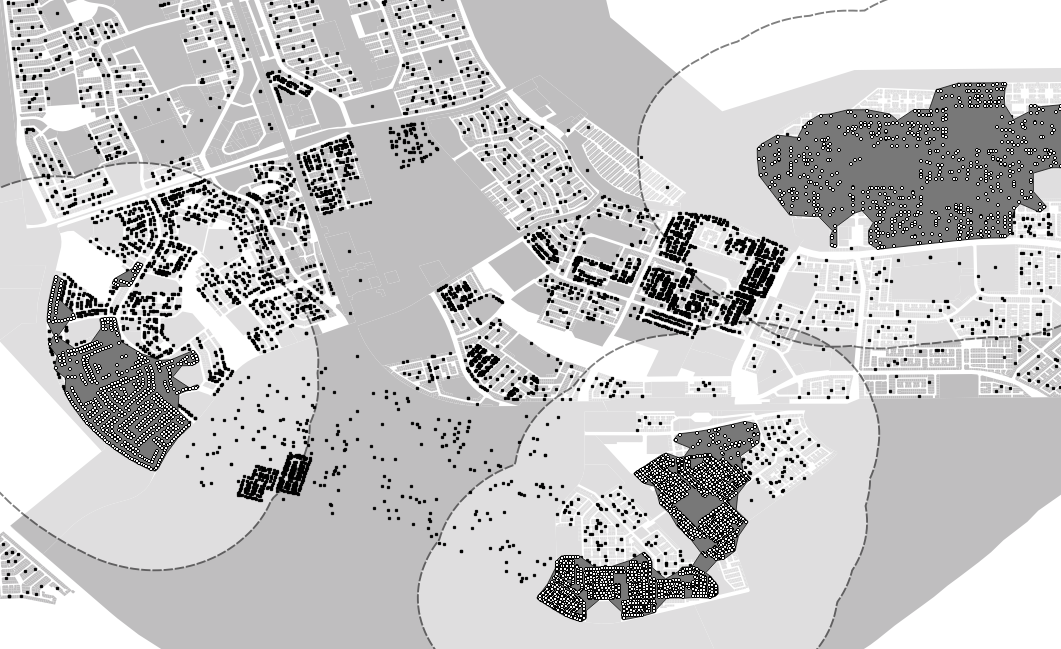
\includegraphics[scale=0.30]{design2.png}
\vspace{-3mm}
\end{figure}
\end{center}
\end{frame}

%------------------------------------------------


\begin{frame}
\frametitle{Housing Price Descriptives}
\centering
\vspace{.1cm}
\resizebox{.95\textwidth}{!}{  
\begin{tabu}{lccc}
\toprule
 & Outside Buffer & Inside Buffer & Housing Project \\
\midrule
 Purchase Price (Rand)  & 184,199.6  & 205,891.3  & 142,748.8  \\ 
\rowfont{\footnotesize} & [386,165.1]  & [249,590.1]  & [447,771.6]  \\ 
 &  &  &  \\ 
 Plot Size (m3)  & 585.2  & 421.7  & 270.4  \\ 
\rowfont{\footnotesize} & [2,040.3]  & [1,225.7]  & [179.2]  \\ 
 &  &  &  \\ 
 Sold At Least Once  & 0.316  & 0.318  & 0.338  \\ 
 Median Purchase Year  & 2006  & 2006  & 2006  \\ 
 Distance to Project (meters) &  & 373.0  & \\
 \rowfont{\footnotesize} &  & [415.9]  & \\
\midrule
 Observations  & 275,296  & 94,172  & 108,809  \\ 
\bottomrule
\end{tabu}

}
% descriptive_statistics.do program: write_descriptive_table
\end{frame}

%------------------------------------------------


\begin{frame}
\frametitle{Estimating Differences-in-Differences}

\begin{align*}
P_{itp} \, =& \, \sum_{d=1}^{D} \alpha_d \mathds{1}[dist=d] Post_{tp} \, + \sum_{d=1}^{D} \alpha_d \mathds{1}[dist=d] Pre_{tp} \\
& + \, \gamma_t \, + \, \lambda_p \, + \theta X_{i} + \, \varepsilon_{itp} \\
P_{itp} \, =& \, \sum_{e=1}^{E} \alpha_j \mathds{1}[time=e] Near_{tp} + \sum_{e=1}^{E} \alpha_j \mathds{1}[time=e] Far_{tp} \\
& \, + \, \gamma_t \, + \, \lambda_p \, + \theta X_{i} + \, \varepsilon_{btp}
\end{align*}

\begin{itemize}
\item $i$: transaction, $t$: year-month, $p$: project
\item $P_{gtp}$: Purchase price (formal houses)
\item $dist$: dist to project, $Near_{tp}$: $<$400m, $Far_{tp}$: $\geq$400m \& $<$1200
\item $time$: months to project, $Post_{tp}$: 36 months after, $Pre_{tp}$ 36 before
\item $\lambda_p$: project fixed effect, $\gamma_t$: calendar month fixed effect
\end{itemize}


\end{frame}


\begin{frame}
\begin{figure}
\caption{Price Estimates over Distance}\label{figure:distplot}
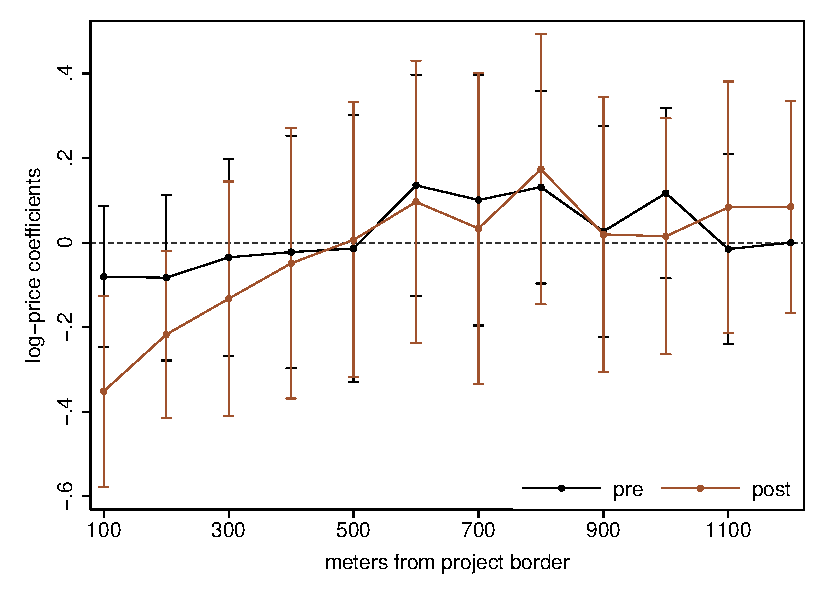
\includegraphics[width=0.5\textwidth,trim={.77cm 0cm .21cm 0cm}]{distplot.pdf}
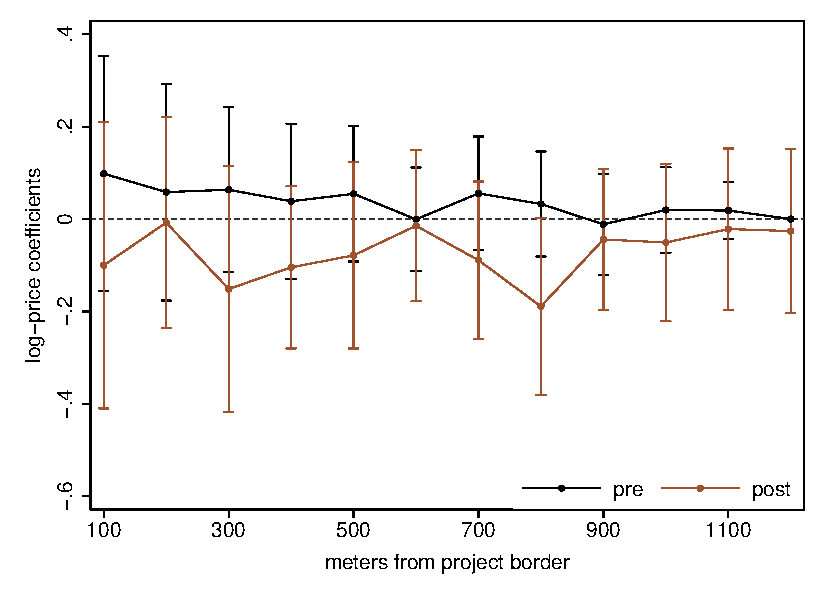
\includegraphics[width=0.5\textwidth,trim={.77cm 0cm .21cm 0cm},clip]{distplot_placebo.pdf}\\
{\color{white}dd}Completed Projects \hspace{4.2cm} Uncompleted Projects
\end{figure}

\end{frame}



\begin{frame}
\begin{figure}
\caption{Price Estimates over Time}\label{figure:timeplot}
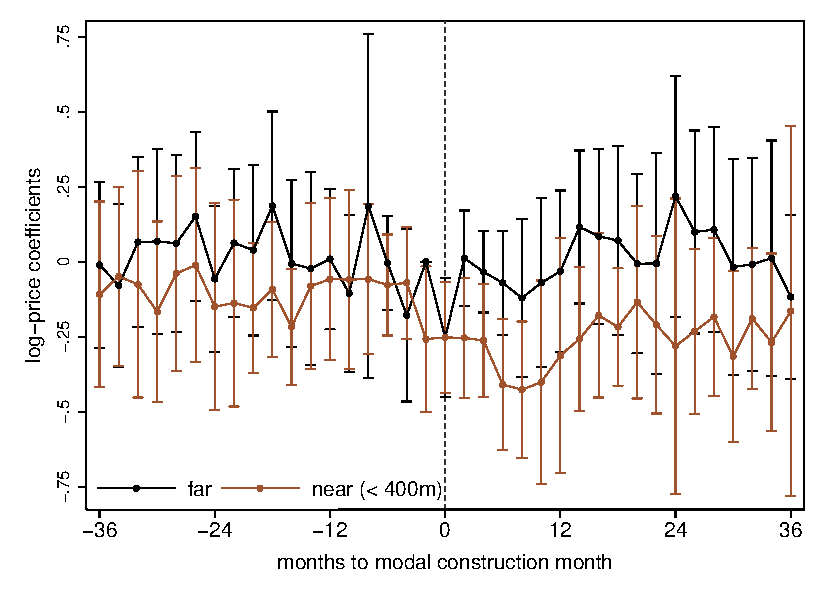
\includegraphics[width=0.5\textwidth,trim={.77cm 0cm .21cm 0cm}]{timeplot.pdf}
   \hfill
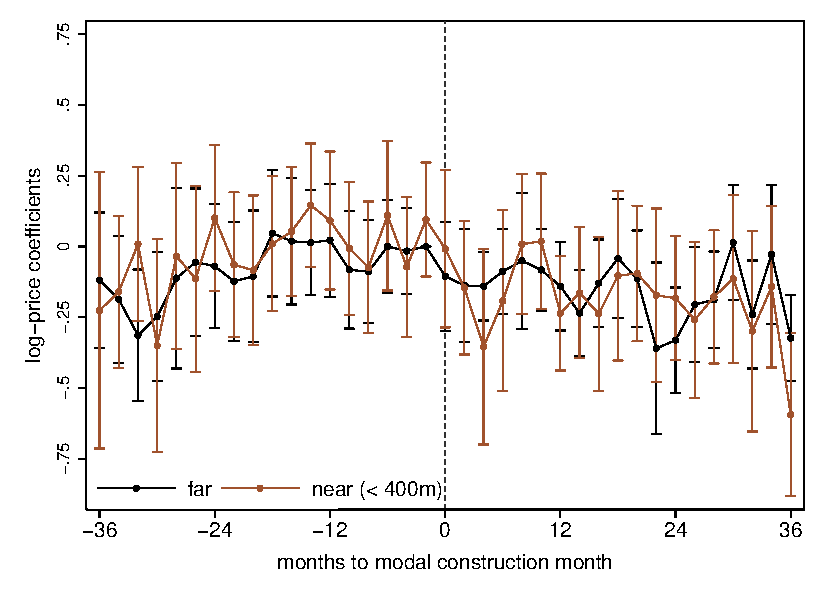
\includegraphics[width=0.5\textwidth,trim={.77cm 0cm .21cm 0cm},clip]{timeplot_placebo.pdf}\\
{\color{white}dd}Completed Projects \hspace{4.2cm} Uncompleted Projects
\end{figure}
\end{frame}
%------------------------------------------------

%% THIS SLIDE INCLUDES THE MATCHING METHOD %% 

%\begin{frame}
%\frametitle{Matching Method}
%\centering
%\begin{tabu}{lcc}
 & Matched  & Unmatched  \\
\midrule
 Formal Density: 2001  & 230.5  & 171.5  \\ 
 Formal Density: 2011  & 814.1  & 444.0  \\ 
 &  &  \\ 
 Informal Density: 2001  & 1,055.6  & 1,401.0  \\ 
 Informal Density: 2011  & 1,613.2  & 2,147.0  \\ 
 &  &  \\ 
 Project House Density  & 125.0  & 66.0  \\ 
 Project Mode Year  & 2005  & 2005  \\ 
 &  &  \\ 
 Hectares  & 97.3  & 119.6  \\ 
 &  &  \\ 
\midrule
 Observations  & 322  & 320  \\ 
\bottomrule
\end{tabu}

%\end{frame}





\end{document} 
